\documentclass{beamer}

\usepackage{amssymb}
\usepackage{epsfig,shadow}
\usepackage{beamerthemeshadow}

\beamertemplatetransparentcovereddynamic
\setbeamertemplate{navigation symbols}{}

%%%%%%%%%%%%%%
% Title page %
%%%%%%%%%%%%%%%%%%%%%%%%%%%%%%%%%%%%%%%%%%%%%%%%%%%%%%%%%%%%%%%%%%%%%%%%%%%%%%%

\title[OAR2]{
    OAR2\\
    An open source resource manager for large clusters
}
\author[Mescal/ID]{
    {\bf Mescal/ID}\\
    {\tiny Joseph.Emeras@imag.fr Nicolas.Capit@imag.fr Olivier.Richard@imag.fr
            Yiannis.Georgiou@imag.fr}
}

\institute{
    \begin{center}
        \includegraphics[height=16ex]{src/img/oar_logo.png}
    \end{center}
    {\bf http://oar.imag.fr/}
    \begin{center}
        %\vspace{2ex}
        
\includegraphics[height=9ex]{src/img/LIG_coul.jpg}
        \hspace{2ex}
        
\includegraphics[height=5ex]{src/img/cnrs.jpg}
        \hspace{1ex}
        
\includegraphics[height=5ex]{src/img/logo_inpg.jpg}
        \hspace{1ex}
        
\includegraphics[height=5ex]{src/img/inria.jpg}
        \hspace{1ex}
        
\includegraphics[height=5ex]{src/img/logo_ujf.jpg}
        \hspace{1ex}
        
\includegraphics[height=5ex]{src/img/logo_upmf.jpg}
    \end{center}
}
\date{{\tiny \today}}

\begin{document}

\frame[plain]{\titlepage}

%%%%%%%%%%%%%%%%%%%%%
% Table of contents %
%%%%%%%%%%%%%%%%%%%%%%%%%%%%%%%%%%%%%%%%%%%%%%%%%%%%%%%%%%%%%%%%%%%%%%%%%%%%%%%

\frame{
    \frametitle{Part I: Production versions}
    \tableofcontents[pausesections,part=1]
}

\frame{
    \frametitle{Part II: Research}
    \tableofcontents[part=2]
}

%%%%%%%%%%%%%%
% First part %
%%%%%%%%%%%%%%%%%%%%%%%%%%%%%%%%%%%%%%%%%%%%%%%%%%%%%%%%%%%%%%%%%%%%%%%%%%%%%%%
\part{Production versions}
\frame{\partpage}

\section{Introduction}
        \frame{
            \frametitle{What is OAR designed for (1)}
            OAR is an open source batch/resource manager for clusters.\\
            \bigskip
            Historically: created to replace PBSpro on the Icluster (begun non free for universities).\\
            \bigskip
            OAR:
            \begin{itemize}
                \item Use {\bf OpenSSH} daemon on compute nodes.
                \item Batch or interactive jobs.
                \item {\bf Gantt} scheduling (with reservations).
                \item No dependence on specific computing libraries like MPI.
                \item 2 web interfaces (Monika and DrawGantt).
            \end{itemize}
        }
        \frame{
            \frametitle{What is OAR designed for (2)}
            \begin{center}
                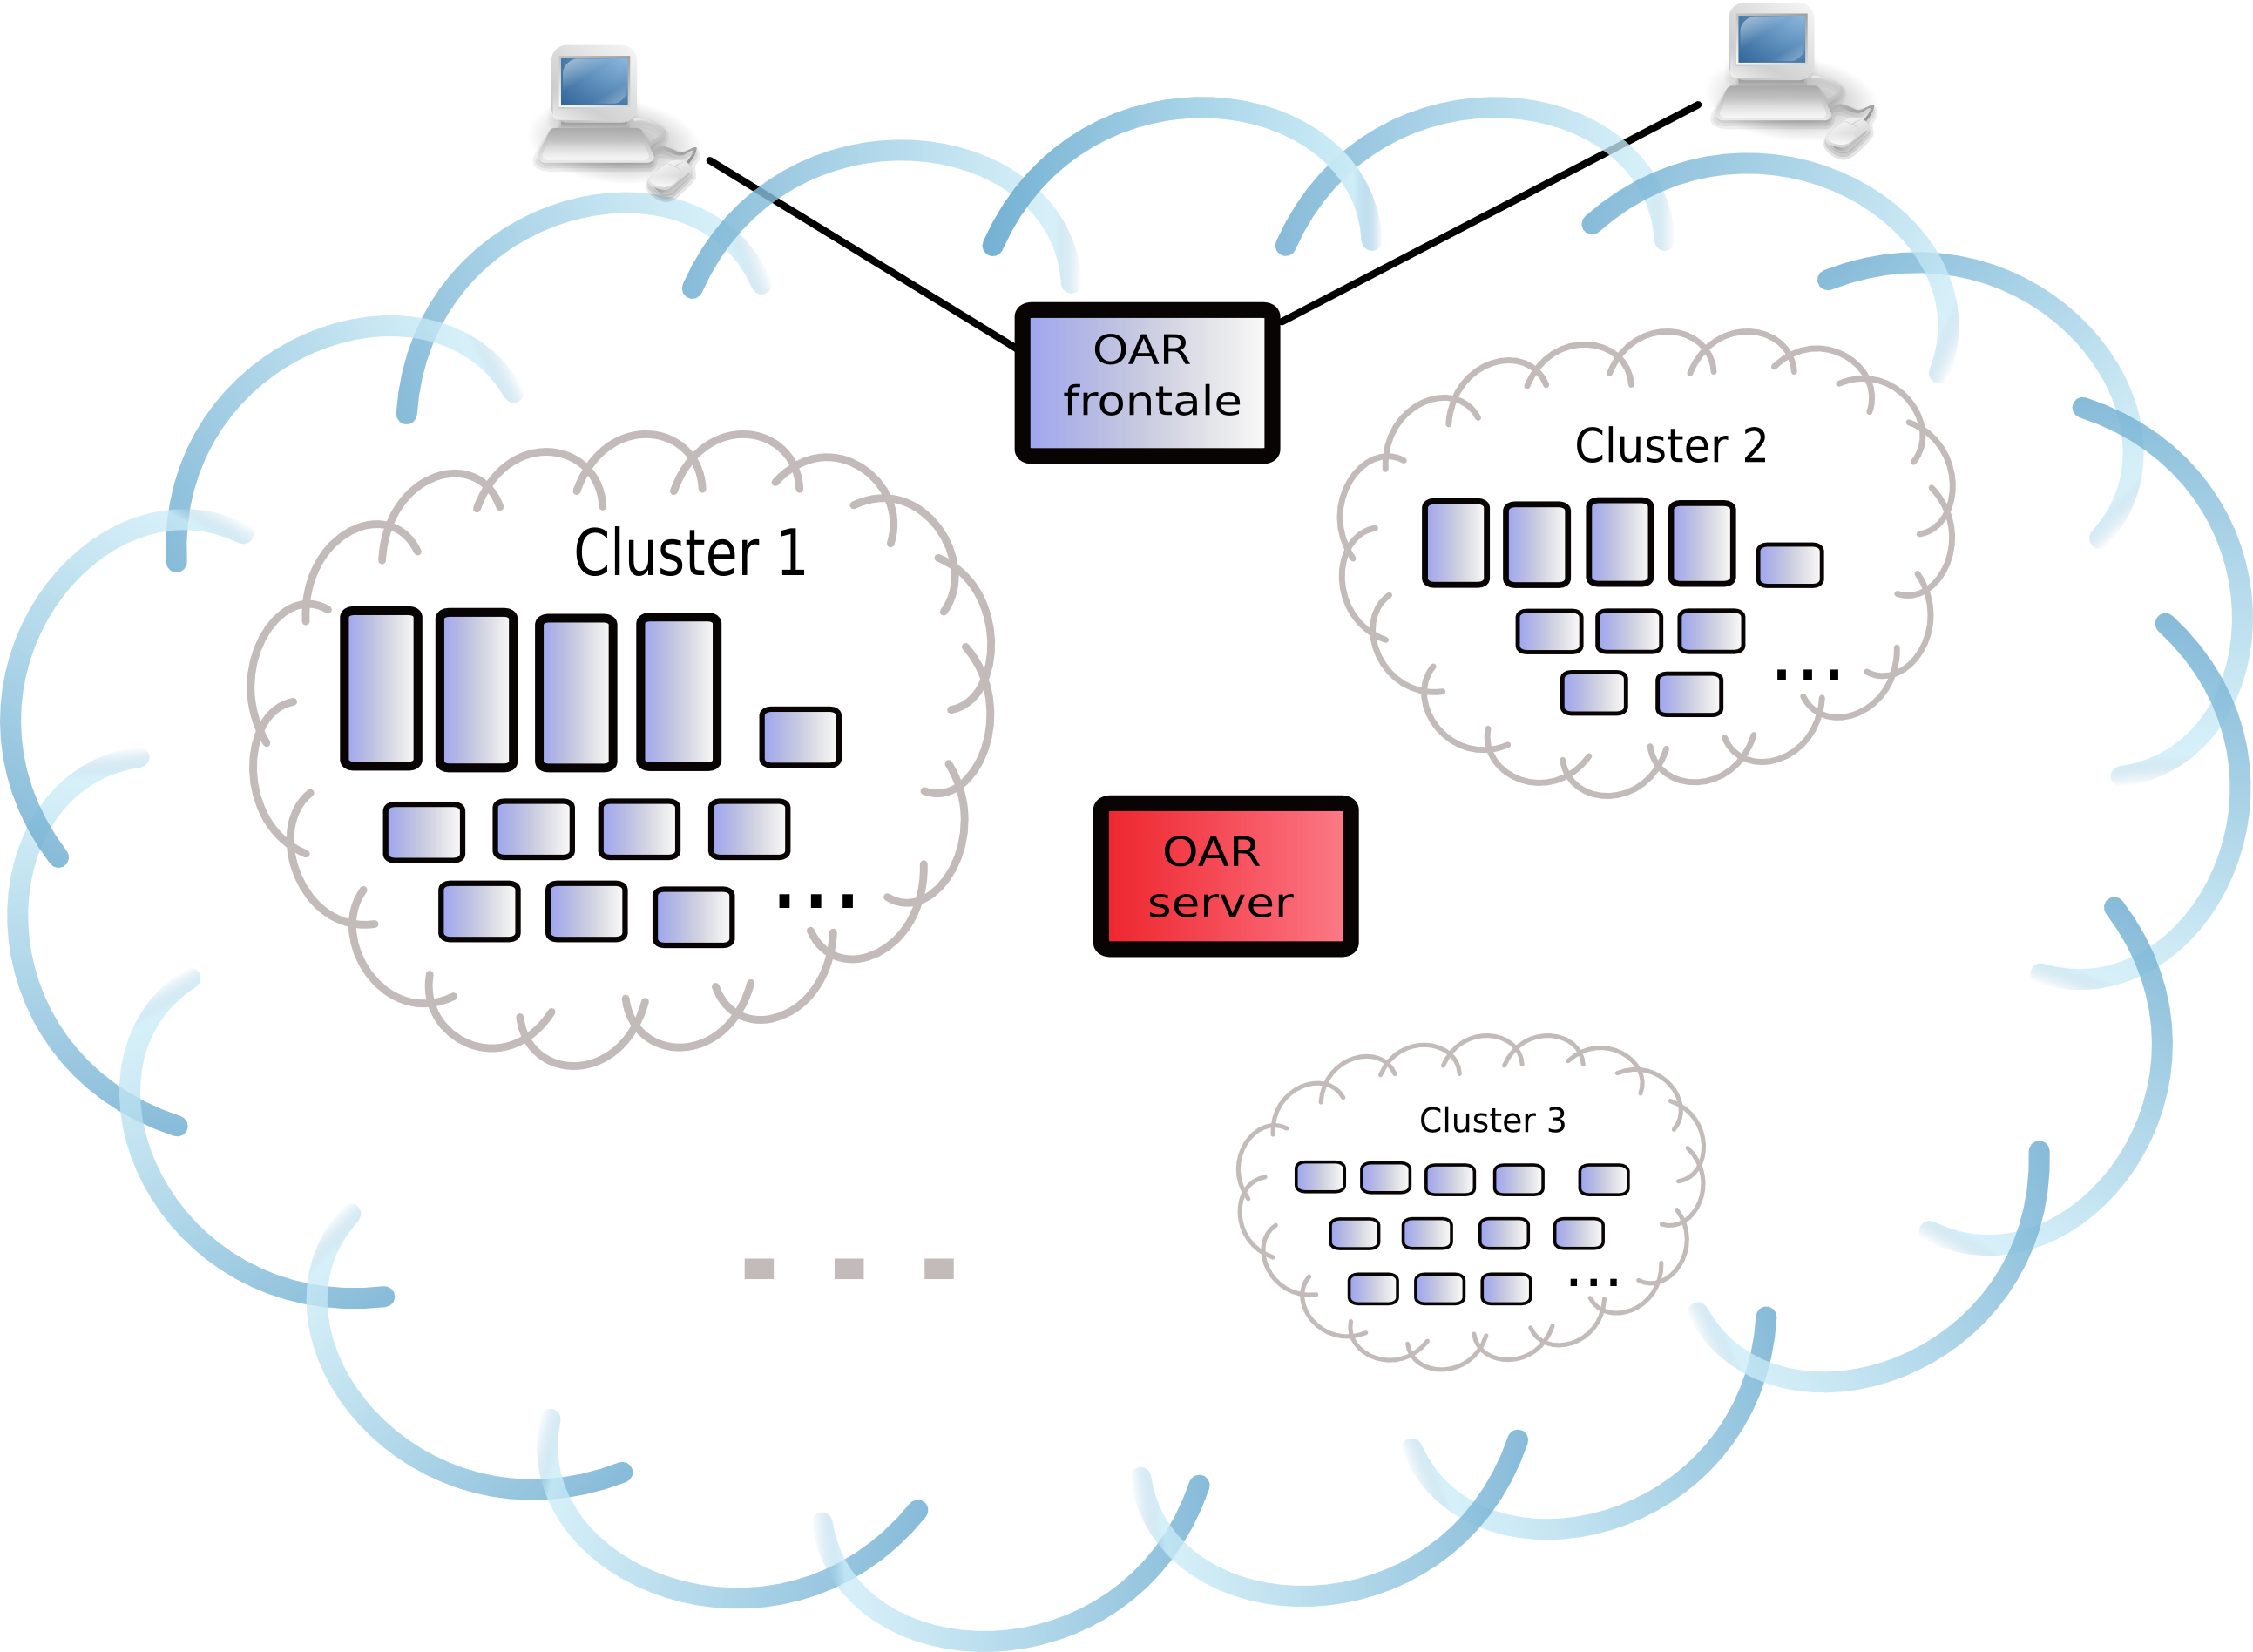
\includegraphics[height=40ex]{src/img/clusters_intro.png}
            \end{center}
        }
        \frame{
            \frametitle{OAR2 enhancements}
            OAR2 is a huge rewrite of the first version:
            \begin{itemize}
                \item Manage {\bf heterogeneous} clusters.
                \item Solution to {\bf clean} properly compute nodes.
                \item Support of dynamic nodes.
                \item Support moldable jobs.
                \item Support job types.
                \item Suspend/resume job execution.
                \item Fair sharing scheduler algorithm.
                \item ...
            \end{itemize}
        }

\section{Strong concepts}
    \subsection{Modules around a database}
        \frame{
            \frametitle{Modules around a database}
            Everything is stored in a {\bf database} (PostgreSQL or MySQL).\\
            This is the only way of communication between each functional modules.\\
            \begin{itemize}
                \item Advantages:
                    \begin{itemize}
                        \item Simplicity.
                        \item Choose your language to write the modules (currently in Perl).
                        \item Able to use database technologies for the replication, backup, mirroring, ...
                    \end{itemize}
                \item Drawback:
                    \begin{itemize}
                        \item Huge amount of database requests.
                    \end{itemize}
            \end{itemize}
            \bigskip
            So everything is logged and can be post-treated by other tools.
        }
        \frame{
            \frametitle{Database scheme}
            \begin{center}
                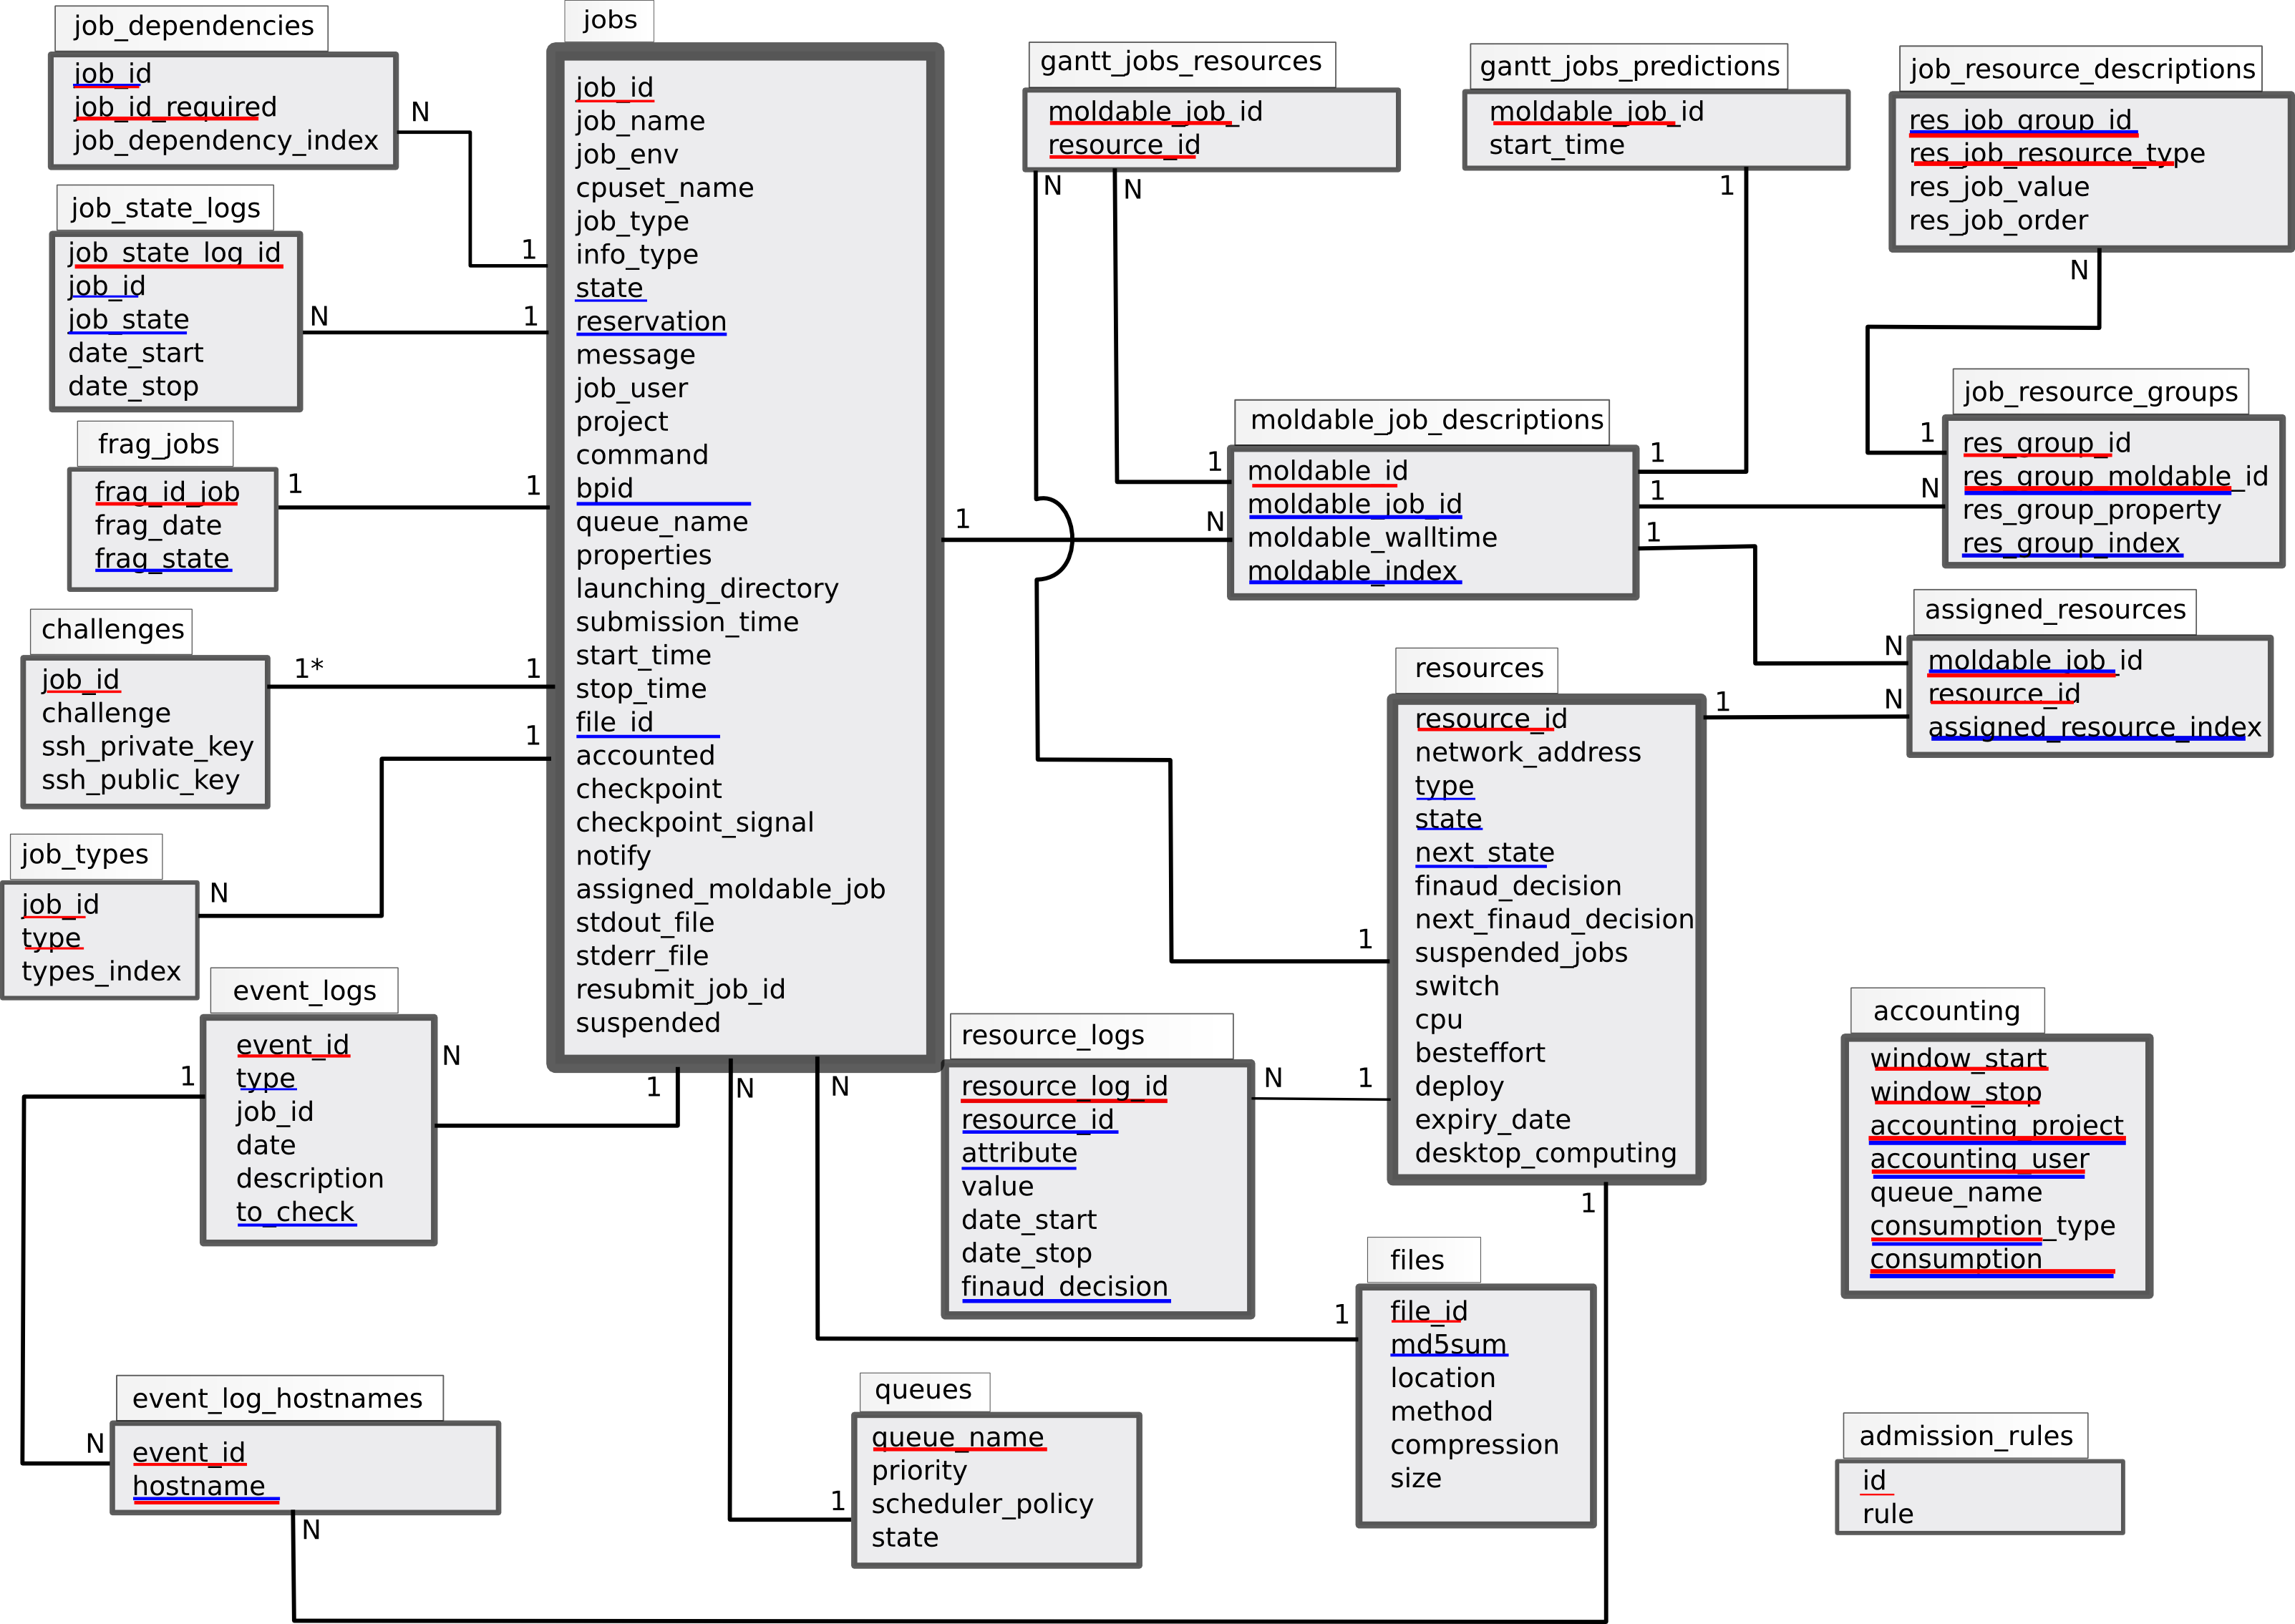
\includegraphics[height=40ex]{src/img/db_scheme.png}
            \end{center}
        }
    \subsection{Hierarchical resources}
        \frame{
            \frametitle{Resources}
                Everything is a {\Large resource}(or a set of resources):
                \begin{itemize}
                    \item compute nodes
                    \item CPUs
                    \item CPU cores
                    \item memory slots
                    \item licences (MathLab, Fluent, ...)
                    \item ...
                \end{itemize}
            By default a resource = part of a node.\\
            OAR2 uses these data in a hierarchical manner.
        }
        \frame{
            \frametitle{The hierarchies}
            Not only 1 hierarchy but everything the users want.\\
            Depends on what the administrator fills in the database.\\
            For example:
            \begin{itemize}
                \item nodes
                \item cpus $>$ nodes
                \item cores $>$ cpus $>$ nodes $>$ switches $>$ clusters
                \item cores $>$ switches
                \item ...
            \end{itemize}
        }
        \frame{
            \frametitle{Graphical example}
            \begin{center}
                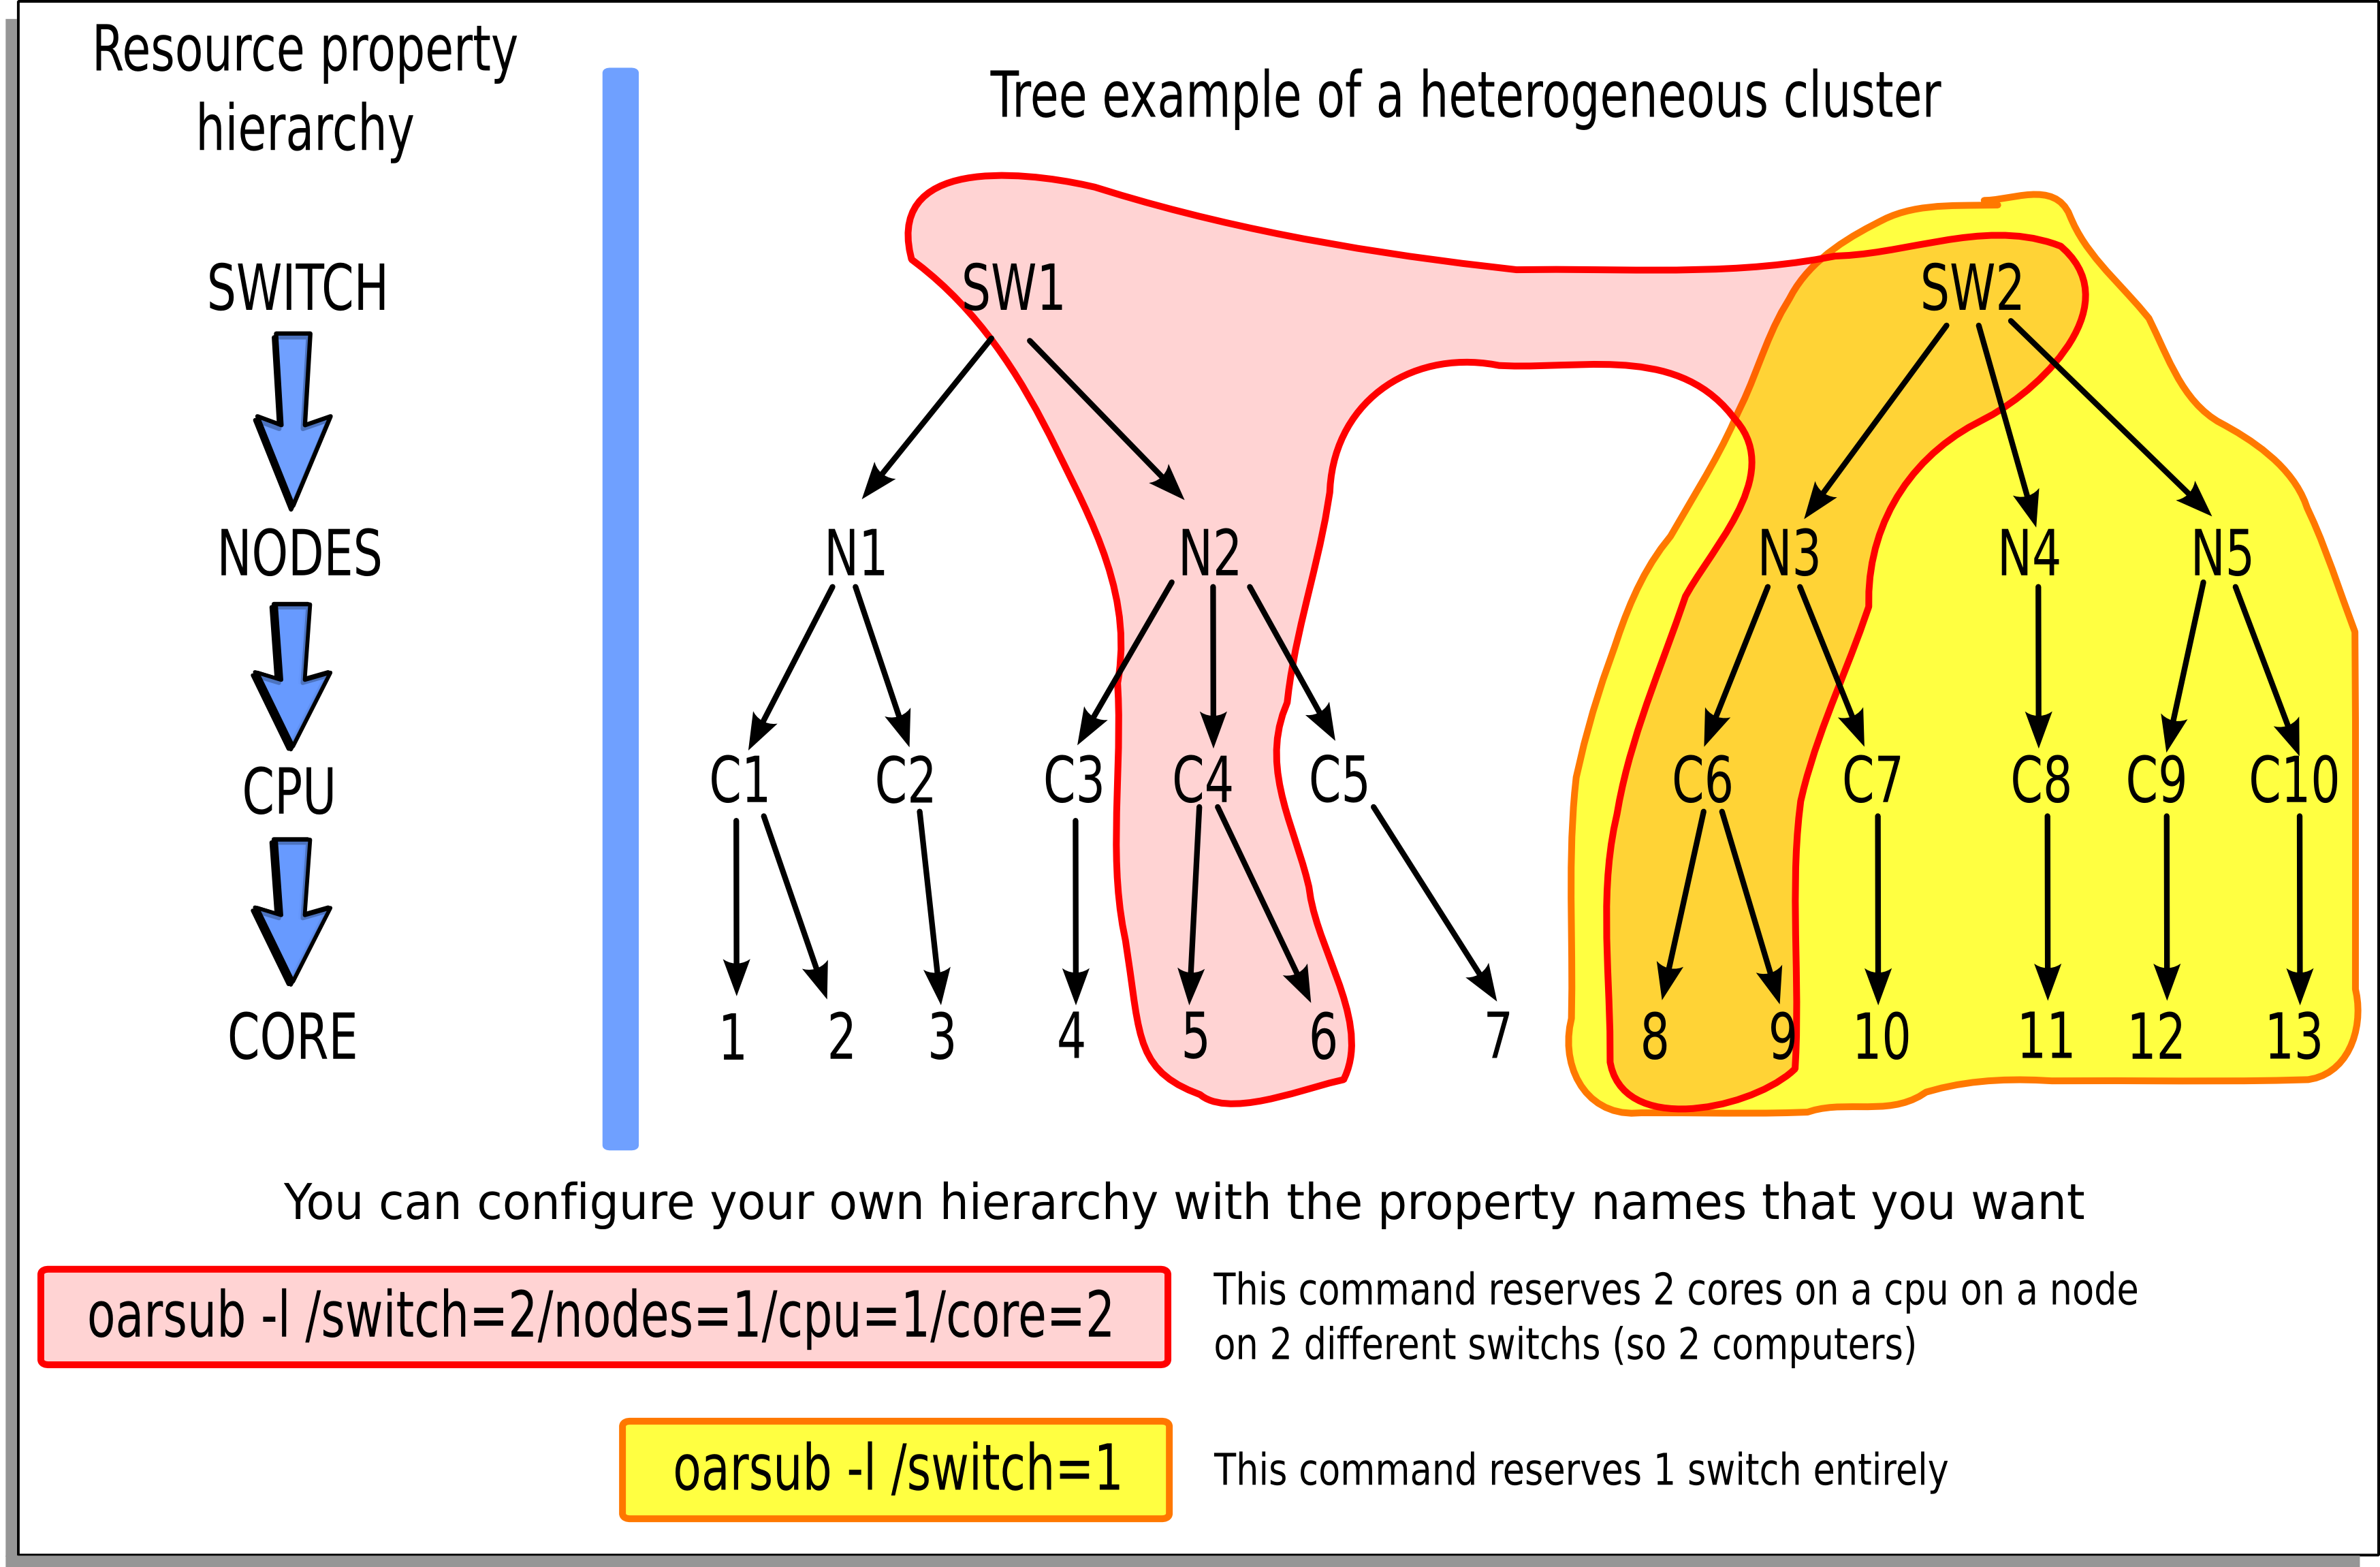
\includegraphics[height=40ex]{src/img/hierarchical_resources.png}
            \end{center}
        }
    \subsection{oarsh}
        \frame{
            \frametitle{oarsh/oarsh\_shell}
            Wrapper around the {\Large ssh} command.\\
            Only way to {\bf connect} from one compute node to an other.
            \begin{itemize}
                \item Advantages
                    \begin{itemize}
                        \item OAR manages user connections.
                        \item The users don't need anymore to configure their SSH keys.
                        \item Transfer automatically jobs information (CPUSET, user id).
                        \item Can use oarsh like ssh (for example: "-X" is working).
                        \item The users are not able to log on unreserved resources.
                    \end{itemize}
                \item Drawback
                    \begin{itemize}
                        \item The users have to use oarsh in their program to log on the nodes (replace ssh by oarsh).\\
                        {\tiny But there is a solution if it is not possible (see "job key" subsection).}
                    \end{itemize}
            \end{itemize}
        }
        \frame{
            \frametitle{CPUSETs}
            Mechanism for assigning a set of CPUs and Memory Nodes to a set of tasks.\\
            (this functionality is included in 2.6 Linux kernels)\\
            \bigskip
            OAR creates 1 CPUSET per job on {\bf each} reserved nodes.\\
            Then it fills CPUs and Memory Nodes with the right value (from the database resources).\\
            \bigskip
            The CPUSET name is propagated via {\bf oarsh} on each nodes. So the
            users cannot go out of their CPUSET during a job.
        }
        \frame{
            \frametitle{CPUSET advantages}
            \begin{itemize}
                \item {\bf Restricts} the use of the Cpus and Memory.
                \item Very useful on big NUMA nodes but not only...
                \item Keeps the {\bf list} of every child {\bf processes} of a job.\\
                      So it is possible to track job user forks and then to
                      {\bf clean} (kill remaining processes) all the nodes after the
                      end of the job.
            \end{itemize}
            \bigskip
            {\Large This is a really huge enhancement in the OAR job clean process.}
        }
        \frame{
            \frametitle{job key}
            Concept: assign a {\bf SSH key} for each OAR job.\\
            \bigskip
            \begin{itemize}
                \item The users are able to use this key to connect to all
                      nodes of their job via the {\tt normal} {\bf ssh} command
                      ("-i" option).
                \item {\bf Grid} usage: can use the same job key on 2 OAR server
                      on 2 different clusters and then connect to the whole nodes.\\
                      Once submitted with the same job key, the connections are
                      completely transparent via "oarsh".
            \end{itemize}
        }
        \frame{
            \frametitle{job temporary user (1)}
                From now,\\
                the best {\bf container} on every UNIX systems is the {\Large user id}:
            \begin{itemize}
                \item processes
                \item files
                \item sockets
                \item IPC (shared memory)
                \item ...
            \end{itemize}
        }
        \frame{
            \frametitle{job temporary user (2)}
            Idea:
            \begin{enumerate}
                \item Add a pool of temporary user id in the resources.
                \item Reserve automatically one of these user id when submitting a new job.
                \item At the beginning of the job, just create the temporary user.
                \item At the end of the job, clean everything you want from this temporary user and then delete it.
            \end{enumerate}
            Drawbacks:
            \begin{itemize}
                \item Each user must have an unique primary group.
                \item The same temporary user id can be used by different users
                      (not at the same time). So be careful with file
                      permissions.
            \end{itemize}
            $\Rightarrow$ it depends of the distributed file system used.
        }
    \subsection{Scalability}
        \frame{
            \frametitle{Taktuk}
            External command ({\tt http://taktuk.gforge.inria.fr/}):
            \begin{itemize}
                \item Performs large scale remote execution deployment.
                \item Platform independent.
                \item Not needed to install it on compute nodes.
                \item I/O redirection
                \item Sliding window + tree diffusion (uses work-stealing) algorithm.
                \item Uses a generic connector like ssh, rsh, ... (here it is ssh).
            \end{itemize}
            Every OAR node management actions are performed via the Taktuk command.\\
        }
        \frame{
            \frametitle{Taktuk example}
            \begin{center}
                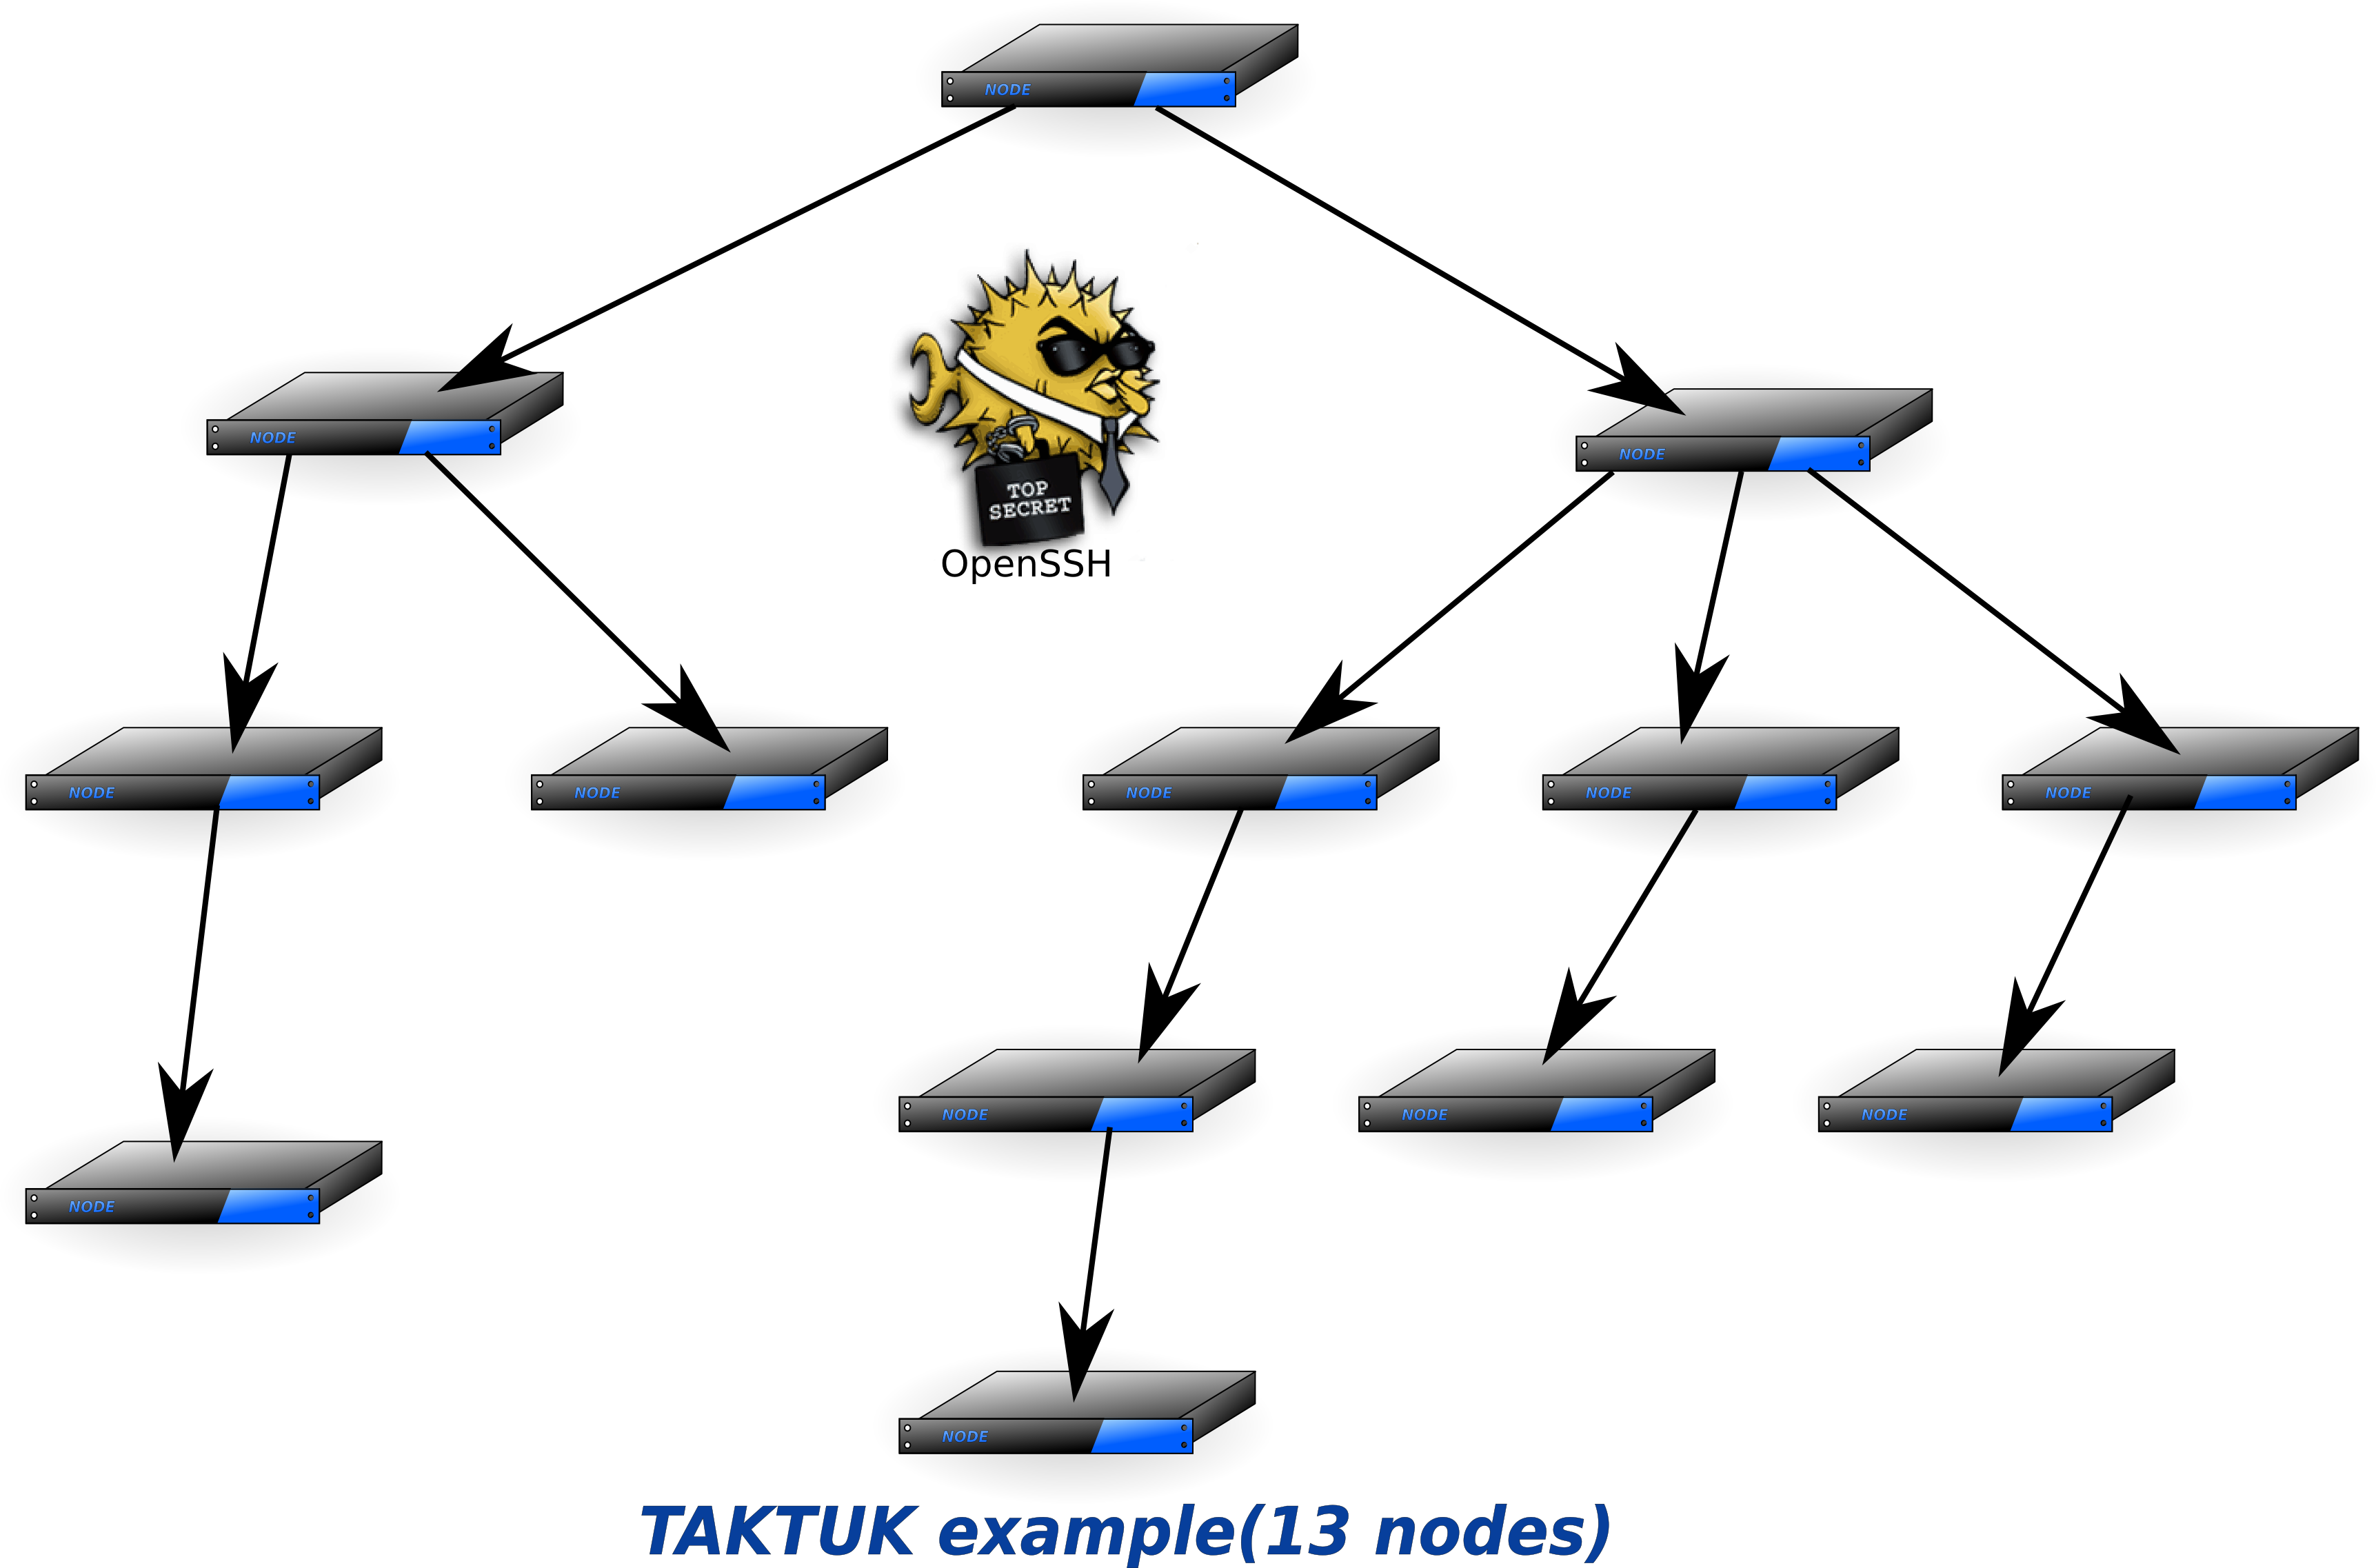
\includegraphics[height=40ex]{src/img/taktuk.png}
            \end{center}

        }
        \frame{
            \frametitle{Scheduling}
            \begin{itemize}
                \item Every possibilities = impossible
                \item hierarchical job resource description = make the work of the scheduler easier and more scalable
            \end{itemize}
            \bigskip
            Can be implemented with another programming language.
        }

\section{Functionalities}
    \subsection{Administrator side}
        \frame{
            \frametitle{Administrator functionalities}
            \begin{itemize}
                \item Add/remove resources.
                \item Add/remove resource properties.
                \item Change property values of resources.
                \item Manage scheduling queues (priority, scheduler).
                \item Suspend/resume jobs.
                \item Change admission rules.
                \item Configure dynamic nodes (save power by switch on only right nodes and switch off the others).
            \end{itemize}
        }

    \subsection{User side}
        \frame{
            \frametitle{Monika}
            \begin{center}
                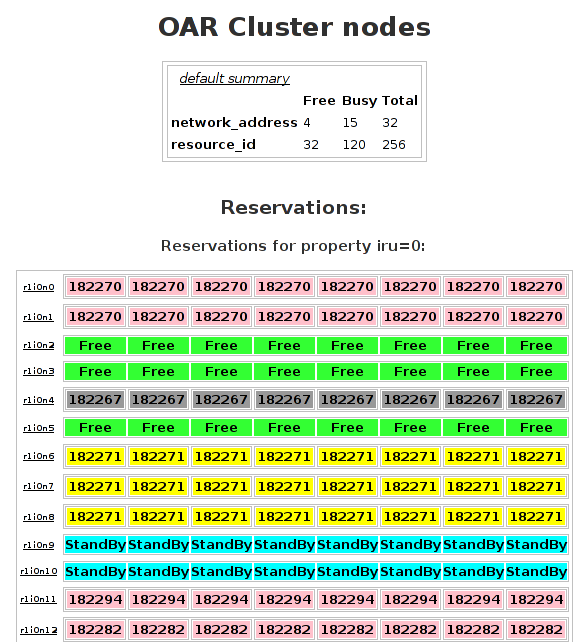
\includegraphics[height=40ex]{src/img/monika.png}
            \end{center}
        }
        \frame{
            \frametitle{DrawGantt}
            \begin{center}
                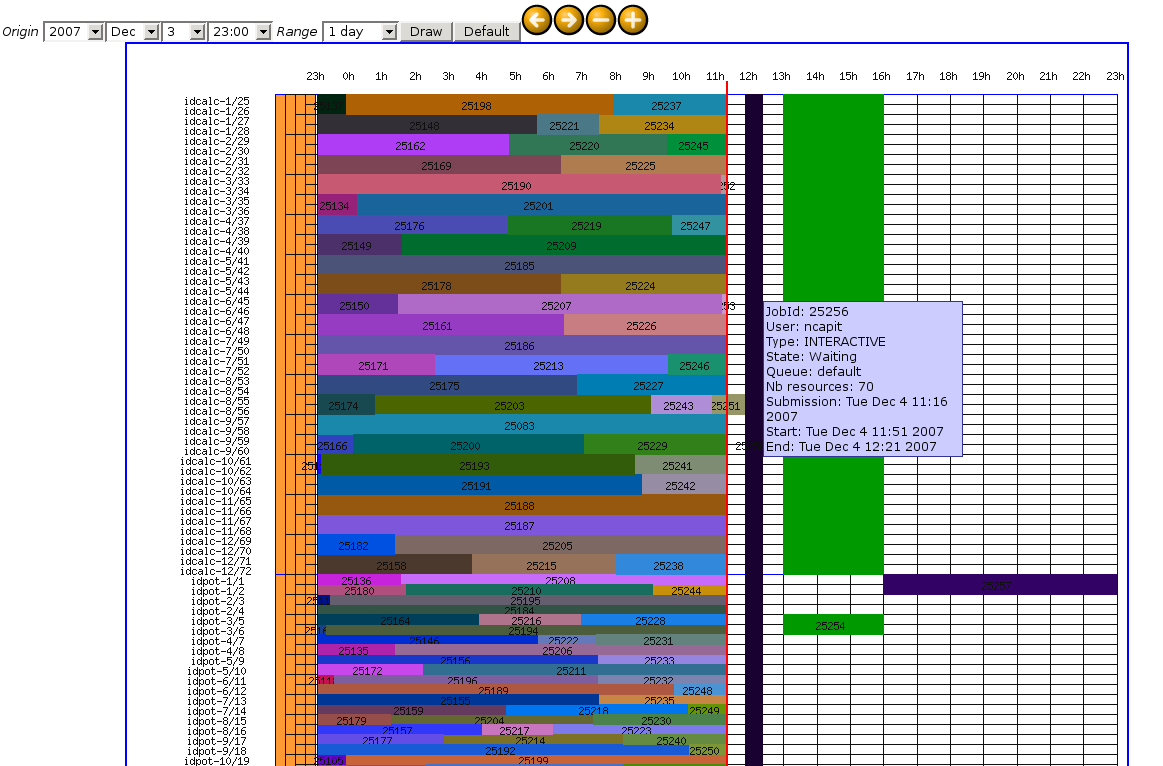
\includegraphics[height=40ex]{src/img/drawgantt.png}
            \end{center}
        }
        \frame{
            \frametitle{User functionalities}
            \begin{itemize}
                \item Reservations.
                \item Moldable jobs.
                \item Timesharing.
                \item Besteffort jobs.
                \item Checkpoint notification.
                \item Change default stdout and stderr files.
                \item Job dependencies.
                \item Notification (start and end of the job).
                \begin{itemize}
                    \item Send emails.
                    \item Execute a program on the frontale.
                \end{itemize}
                \item Resubmission.
            \end{itemize}
            {\tiny All user commands have a XML, YAML and Perl DUMPER output format}
        }

    \subsection{Simple use cases}
        \frame[containsverbatim]{
            \frametitle{Simple use cases (1)}
\begin{verbatim}
oarsub -I

oarsub -I -l nodes=3,walltime=2:00:00

oarsub -l nodes=3,walltime=2:00:00 ./prog.sh

oarsub -I -l core=43

oarsub -I -l nodes=40/cpu=4

oarsub -I -l switch=3/nodes=1

oarsub -I -l nodes=10 -p "mem >= 512"
\end{verbatim}
        }
        \frame[containsverbatim]{
            \frametitle{Simple use cases (2)}
\begin{verbatim}
oarsub -r "2008-01-10 18:00:00"\
-l nodes=120,walltime=48:00:00

oarsub -r "2008-01-10 18:00:00"\
-l nodes=120,walltime=48:00:00 ./prog.sh

oarsub -I -a 4256 -a 4257 -l switch=1

oarsub --notify "mail:capitn@imag.fr" ./prog.sh

oarsub --notify "exec:/path/to/user/job.sh" ./prog.sh

oarsub -l core=1,walltime=1:0:0 --checkpoint 900\
--signal 15 ./checkpoint.sh
\end{verbatim}
        }

    \subsection{More complex use cases}
        \frame[containsverbatim]{
            \frametitle{More complex use case}
\begin{verbatim}
oarsub --checkpoint 600 --signal 2 -t idempotent ./prog.sh

oarsub -t besteffort -t idempotent -l cpu=1 ./prog.sh

oarsub -l nodes=20/core=1 'taktuk -c "oarsh"\
-f $OAR_FILE_NODES broadcast exec [ date ]'

oarsub -l cpu=2,walltime=16 -l cpu=4,walltime=8\
-l cpu=8,walltime=4 ./moldable_prog.sh

oarsub -I -l "{mem = '32G' or mem = '64G'}/cpu=1+/cpu=32"

oarsub -I\
-l "/switch=2/nodes=10+{type = 'mathlab'}/licence=20"
\end{verbatim}
        }

\section{OAR2 in action}
    \frame{
        \frametitle{Current installations (1)}
        OAR2 is ready for production and is already installed in:
        \begin{itemize}
            \item the {\large CIMENT} project ({\tt https://ciment.ujf-grenoble.fr/})\\
                  almost 500 cores in 9 different clusters
            \item the {\large GRID5000} project ({\tt https://www.grid5000.fr/})\\
                  9 sites (with 1 OAR server per site)\\
                  more than 3000 cores in 20 clusters
        \end{itemize}
    }
    \frame{
        \frametitle{Current installations (2)}
            \begin{itemize}
                \item from Poland ({\tt http://www.ioe.wat.edu.pl/})
                \item from the University of Michigan
                \item from a french bank
                \item ...
            \end{itemize}
    }
    \frame{
        \frametitle{Versioning}
        The current {\bf stable branch} is the {\bf 2.2}.\\
        The third digit is used to bring out only bug fix released.\\
        \bigskip
        The version under development is the 2.3.\\
        \bigskip
        Other branches can be used for research oriented experimentations.\\
        \bigskip
        For sources,Debian packages and USB live key images:\\
        \bigskip
        \hspace{4ex}{\tt http://oar.imag.fr/download.html}
    }

%%%%%%%%%%%%%%%
% Second part %
%%%%%%%%%%%%%%%%%%%%%%%%%%%%%%%%%%%%%%%%%%%%%%%%%%%%%%%%%%%%%%%%%%%%%%%%%%%%%%%
\part{Research}
\frame{\partpage}

\frame{
    \frametitle{Part II: Research}
    \tableofcontents[pausesections,part=2]
}

\section{Resource Management Systems: Evaluation Methodology}
\frame{
    \frametitle{RMS: Theoretical Comparaison}
            \begin{itemize}
                \item Identity Classification
		\item Functionalities Comparaison
		\item Based on Projects Documentation
            \end{itemize}
\href{http://oar.imag.fr/rms_comparison_tables3.html}
{{\color{blue} Resource Management Systems Comparaison Table} }
	
}

\frame{
    \frametitle{RMS: Performance Evaluation Values}
           Define What to compare?
            \begin{enumerate}
                \item Nodes-Jobs Scalability
		\item Scheduler Efficiency
		\item Parallel jobs treatment 
		\item ....
            \end{enumerate}
}

\frame{
    \frametitle{RMS: Performance Evaluation Methods}
           Define How to compare? ---: Games of Tests
            \begin{enumerate}
                \item Game of simple similar tests/RMS configurations
		\begin{itemize}
			\item Random Job generation and Submission 
			\item Based on known clusters Workload Traces
		\end{itemize}
		\item Effective System Performance Benchmark (ESP)
		\item Hybrid method (definition of a new ESP...??)
            \end{enumerate}
}

\frame{
    \frametitle{Experimentation Methodology}
\begin{itemize}
\item \textbf{Grid5000} experimental grid platform: direct experimentation
\item Experimentation of different RMS in real-life: \textbf{controlled} and thus \textbf{reproducible} experiments 
\begin{itemize}
\item Image containing all the RMS to be evaluated along with the tests to be launched 
\item Image deployed on desired number of Grid5000 ...Cluster RMS configured
\item Play Games ... Evaluate Real-life values (ex. overheads, NFS streching, database reaction, scheduler efficiency, ...)
\item Collect Results
\end{itemize}
\item Automatic experimentation driven by bash scripts
\item Methodology constructed and validated for the study of a lightweight grid CIGRI (ref: escience2007)
\end{itemize}
}


\section{Integrating SLURM with OAR2}
\frame{
    \frametitle{SLURM Description}
SLURM Basic Resource Management System key features:
\begin{itemize}
\item Highly scalable
\item Fault tolerant
\item Basic queue and batch scheduler
\item API for scheduler integration (Maui,Moab,LSF)
\end{itemize}
 
}

\frame{
    \frametitle{Integration Concepts}
Interest of SLURM-OAR2 integration...
\begin{itemize}
\item Can the 2 systems really complement one another?
\item Does SLURM need a better queue and batch scheduler?
\item Is OAR not scalable and efficient resource manager?
\end{itemize}
}

\frame{
    \frametitle{Ways of integration}
\begin{enumerate}
	\item Use the OAR2 scheduler on top of SLURM
	\begin{itemize}
		\item Drawback : Skips all the advantages of OAR2 queue management system (ex. multiple queues, moldable jobs, cosystem jobs)
		\item Easier approach: Rewrite the OAR2 Scheduler using SLURM API
	\end{itemize}
	\item Replace a part of the resource management engine of OAR with SLURM  
	\begin{itemize}
		\item SLURM/srun in the place of Taktuk/SSH engine
		\item Desactivate OAR2 cpusets, use SLURM cpusets
	\end{itemize}
\end{enumerate}

}


\section{Evolving/Malleable applications}
\frame{
    \frametitle{Definition-Concepts}
Parallel jobs Classification (Feitelson97)
\begin{figure}[tp]
\begin{center}
{\footnotesize{
\hspace{-0.5cm}
\begin{tabular}{|l|l|l|}
\hline  
who decides (number)/ when is it decided & at submission & during submission \\
\hline 
User & \textbf{Rigid} & \textbf{Evolving} \\
\hline 
System & \textbf{Moldable} & \textbf{Malleable} \\
\hline
\end{tabular}
}}
\vspace{-0.2cm}
\end{center}
\end{figure}

}

\frame{
    \frametitle{Problem definition}
	Problems concerning the \textcolor{red}{Resource management system}:
	\begin{itemize}
		\item Theoretically the RMS system can support malleable jobs for full system flexibility to improve the overall system utilization
			but in practice it is a very complicated task for the scheduler.
		\item A lot of theoretical Related Work for malleable jobs
		\item Need of a practical study with real-life experimenation...
		\item Need of concrete Use Cases (real scientific malleable applications)
	\end{itemize}

	
}

\frame{
    \frametitle{Problem definition}
	Problems concerning the \textcolor{red}{Parallel Applications:}
	\begin{itemize}
		\item How to modify a rigid/moldable parallel application to be malleable?
		\item Related work: \textcolor{blue}{Co-Design} of the programming environment and the resource management system.
		\item Need of a simpler method...?
	\end{itemize}
}


\frame{
    \frametitle{Ideas for Ongoing Work}
        \begin{itemize}
		\item Techniques and Strategies for scheduling efficiently malleable jobs 
			without changing the resource manager... use of already existing features:
		\begin{itemize}
			\item Timesharing 
			\item Backfilling 
			\item Checkpoint-Restart
			\item Suspend-Resume
			\item Combinations
		\end{itemize}
		\item Techniques for transforming a parallel appllication into malleable
		\begin{itemize}
			\item Problem of LAM-MPI...
		\end{itemize}
	\end{itemize}

}


\end{document}

